% ============================================================================
%  Ansatz Expressivity and Symmetry Accounting in a 10- and 12-Qubit
%  LiH Benchmark
%
%  Compile:  pdflatex main.tex     (run twice: ToC + cross-references)
%  No bibtex pass required -- the bibliography is inline.
%  Figures expected in ./figures/
% ============================================================================
\documentclass[11pt,a4paper]{article}

\usepackage[T1]{fontenc}
\usepackage[utf8]{inputenc}
\usepackage{lmodern}
\usepackage[margin=2.4cm,headheight=14pt]{geometry}
\usepackage{amsmath,amssymb}
\usepackage{graphicx}
\usepackage{booktabs}
\usepackage{array}
\usepackage{caption}
\usepackage{enumitem}
\usepackage{fancyhdr}
\usepackage{microtype}
\usepackage{xcolor}

\definecolor{NavyLink}{HTML}{1A4C8B}
\definecolor{BoxBlue}{HTML}{EAF1F9}
\definecolor{BoxRule}{HTML}{1A4C8B}
\definecolor{WarnBg}{HTML}{FDF3E7}
\definecolor{WarnRule}{HTML}{9C5B12}
\definecolor{StopBg}{HTML}{F5EEEE}
\definecolor{StopRule}{HTML}{8B1A1A}

\usepackage{tcolorbox}
\usepackage[colorlinks=true,linkcolor=NavyLink,citecolor=NavyLink,
            urlcolor=NavyLink,bookmarksnumbered=true]{hyperref}

% ---------------------------------------------------------------- callouts --
\newtcolorbox{result}[1][]{%
  colback=BoxBlue, colframe=BoxRule, boxrule=0.7pt, arc=1.5pt,
  left=6pt, right=6pt, top=5pt, bottom=5pt,
  fonttitle=\bfseries\sffamily\small, title={#1}}

\newtcolorbox{caution}[1][]{%
  colback=WarnBg, colframe=WarnRule, boxrule=0.7pt, arc=1.5pt,
  left=6pt, right=6pt, top=5pt, bottom=5pt,
  fonttitle=\bfseries\sffamily\small, title={#1}}

\newtcolorbox{unsupported}[1][]{%
  colback=StopBg, colframe=StopRule, boxrule=0.7pt, arc=1.5pt,
  left=6pt, right=6pt, top=5pt, bottom=5pt,
  fonttitle=\bfseries\sffamily\small, title={#1}}

% ---------------------------------------------------------------- layout ----
\pagestyle{fancy}
\fancyhf{}
\fancyhead[L]{\small\itshape Ansatz expressivity and symmetry accounting in LiH/STO-3G}
\fancyhead[R]{\small\thepage}
\renewcommand{\headrulewidth}{0.4pt}

\captionsetup{font=small,labelfont=bf,skip=6pt}
\setlength{\parskip}{0.30em}
\setlength{\parindent}{0pt}

\renewcommand{\topfraction}{0.92}
\renewcommand{\bottomfraction}{0.75}
\renewcommand{\textfraction}{0.06}
\renewcommand{\floatpagefraction}{0.75}
\setcounter{topnumber}{3}
\setcounter{bottomnumber}{2}
\setcounter{totalnumber}{5}
\raggedbottom

% ---------------------------------------------------------------- macros ----
\newcommand{\mHa}{\ensuremath{\,\mathrm{mHa}}}
\newcommand{\Ha}{\ensuremath{\,\mathrm{Ha}}}
\newcommand{\Ang}{\ensuremath{\,\text{\AA}}}
\newcommand{\Ssq}{\ensuremath{\langle \hat{S}^2 \rangle}}
\newcommand{\Nop}{\ensuremath{\langle \hat{N} \rangle}}
\newcommand{\code}[1]{\texttt{\small #1}}

\title{\vspace{-1.1cm}\textbf{Ansatz Expressivity and Symmetry Accounting\\
in a 10- and 12-Qubit LiH Benchmark}\\[0.4em]
\large A hardware-efficient circuit that reaches $3.4\mHa$\\
by leaving the physical sector}
\author{Bhargav Krishna\\\small\texttt{qacd@qimlabs.com}}
\date{\today}

\begin{document}
\maketitle
\thispagestyle{fancy}

% =============================================================== ABSTRACT ===
\begin{abstract}
\noindent
LiH/STO-3G is solved variationally in two active spaces --- CASCI(2e,5o) at 10
qubits and the complete STO-3G space, FCI(4e,6o), at 12 qubits --- with two
ansatz families, and each result is scored against exact diagonalisation of the
identical second-quantised Hamiltonian. The molecular integrals are produced by
a self-contained McMurchie--Davidson STO-3G engine written for this workflow,
so the entire pipeline executes on one machine with no external quantum
chemistry package.

UCCSD reaches $1.6\times10^{-7}\mHa$ of the CASCI reference at 10 qubits and
$0.011\mHa$ of the FCI reference at 12 qubits, in both cases with particle-number
leakage at or below $1.4\times10^{-7}$ and no penalty term doing any work.

The result of interest is negative. A hardware-efficient \code{real\_amplitudes}
circuit, taken from four layers to eight, improves its energy from $20.15\mHa$
to $3.41\mHa$ above the CASCI reference --- an apparent factor of six, at a cost
of $95{,}391$ circuit executions. Measuring two additional expectation values
shows that the improvement is not physical: at eight layers the converged state
carries $\Nop - 2 = 7.1\times10^{-5}$ and $\Ssq = 2.1\times10^{-3}$, which price
out at $2.19\mHa$ against a budget of $0.16\mHa$. The symmetry the circuit broke
is worth more than the error it has left, so the energy is not a LiH energy and
is not comparable to the reference at all. The four-layer run, which is
numerically far worse, is by contrast a valid measurement of an ansatz
limitation. Reported without the symmetry audit, the ordering of those two runs
inverts.

The cost of the instrumentation is two expectation values per converged state.
\end{abstract}

\tableofcontents
\vspace{0.6em}
\hrule
\vspace{0.8em}

% =========================================================== INTRODUCTION ===
\section{Introduction}

\subsection{Motivation}

A variational quantum eigensolver returns a number. Whether that number is an
approximation to a molecular energy depends on a premise that the optimisation
does not check: that the converged state lies in the symmetry sector the
reference energy was computed in. The variational principle
$\langle \psi | \hat H | \psi \rangle \geq E_0$ holds against the global ground
state of $\hat H$, not against the ground state of the $N$-electron, spin-$S$
sector that the chemistry is about. A state which has leaked out of that sector
can sit below the reference while meaning nothing.

LiH/STO-3G is small enough that this can be examined exactly. The full space is
six spatial orbitals holding four electrons; both active spaces used here are
diagonalisable to machine precision, so the reference is not a
higher-level-of-theory estimate but the exact answer for the operator being
measured. Any discrepancy is therefore attributable to the ansatz, the
optimiser, or the symmetry of the converged state --- and the three can be
separated.

\subsection{System and active spaces}

The geometry is the experimental equilibrium bond length
$r_e(\mathrm{LiH}) = 1.5949\Ang$ (Huber and Herzberg, via NIST CCCBDB), rounded
to $1.595\Ang$, in vacuum, closed shell, in the STO-3G basis. It is an
experimental value with a cited source rather than an optimised one, so the
molecule is fixed independently of anything in the solver.

\begin{table}[htbp]
\centering
\caption{The two active spaces. The reference follows the space: with
\code{frozen-core} the target is CASCI(2e,5o), \emph{not} full-space FCI, and an
energy below it is evidence that the state left the two-electron sector rather
than evidence of better chemistry.}
\label{tab:spaces}
\small
\begin{tabular}{lccccc}
\toprule
\code{--space} & Active space & Frozen & Qubits & Pauli terms & Reference \\
\midrule
\code{frozen-core} & CASCI(2e,5o) & Li $1s$ & 10 & 276 & CASCI in that space \\
\code{full}        & FCI(4e,6o)   & ---      & 12 & 631 & FCI in STO-3G \\
\bottomrule
\end{tabular}
\end{table}

Freezing the lithium $1s$ pair costs $0.227\mHa$ of the $20.378\mHa$ of
correlation energy available in the complete space, which is why the smaller
problem is the better-posed one: it removes two qubits and $355$ Pauli terms at
a cost roughly one seventh of chemical accuracy.

\subsection{Scope and claims}

This report makes four claims and declines several others; \S\ref{sec:unsupported}
lists the declined ones.

\begin{enumerate}[leftmargin=1.4em,itemsep=0.15em]
\item UCCSD attains chemical accuracy against exact diagonalisation in both
  active spaces, and does so with particle-number leakage that is
  structural rather than penalised.
\item A hardware-efficient \code{real\_amplitudes} circuit does not, at either
  four or eight layers.
\item The eight-layer improvement over the four-layer run is an artefact of
  symmetry breaking, and is identified as such by two expectation values that
  cost nothing to measure relative to the optimisation itself.
\item The integral engine written for this workflow reproduces published
  LiH/STO-3G RHF and FCI energies, and the second-quantised Hamiltonian it
  produces reproduces the SCF energy on the Hartree--Fock determinant to ten
  decimal places in both active spaces.
\end{enumerate}

\subsection{Principal results}

\begin{result}[Headline]
UCCSD reaches $1.6\times10^{-7}\mHa$ of CASCI at 10 qubits in $48$ seconds and
$641$ circuit executions. The eight-layer hardware-efficient run reaches
$3.41\mHa$ in $1{,}473$ seconds and $95{,}391$ circuit executions, and that
number is not usable: its symmetry contamination prices at $2.19\mHa$, which
exceeds the error it claims to have left.
\end{result}

% =========================================================== METHODOLOGY ====
\section{Methodology}

\subsection{Integral construction}

PySCF publishes no Windows wheel and its source build is unsupported there, so
\code{integrals.py} implements STO-3G one- and two-electron integrals by the
McMurchie--Davidson scheme, together with closed-shell restricted Hartree--Fock,
in NumPy alone. At six basis functions this is a smaller and more auditable
dependency than a Fortran-backed chemistry package. \code{prepare} uses PySCF
when it is importable and this engine otherwise; the engine actually used is
written into the cache as \code{integral\_backend}, so a result always records
its own provenance. Both results reported here carry
\code{integral\_backend: native-sto3g}.

The engine is deliberately narrow: STO-3G, closed shell, $s$ and $p$ functions.
It refuses other bases and unknown elements rather than guessing.

\subsection{Validation protocol}

\code{tests/test\_integrals.py} pins the engine against three independent
references:

\begin{enumerate}[leftmargin=1.4em,itemsep=0.15em]
\item the H$_2$/STO-3G energy tabulated by Szabo and Ostlund;
\item published LiH/STO-3G RHF and FCI energies;
\item the requirement that the Hartree--Fock determinant of the
  \emph{second-quantised} Hamiltonian equal the SCF energy to ten decimal places
  in both active spaces.
\end{enumerate}

The third is the strongest check available without a second chemistry code,
because it ties the CAS transformation, the two-electron integral
transformation and the frozen-core energy together: an error in any one of them
breaks it.

Separately, \code{run.py validate} diagonalises the \emph{penalised} Hamiltonian
exactly and fails if its ground state does not lie in the target electron
sector. It writes a receipt bound by SHA-256 to the cache, the molecular
specification, the workflow source and the penalty settings. \code{run.py vqe}
refuses to start without a matching receipt, so editing any workflow file
invalidates every downstream result rather than silently producing a
mismatched one.

\subsection{Acceptance criteria}
\label{sec:criteria}

A run is recorded as \code{verified\_chemical\_accuracy} only if all three hold:

\begin{enumerate}[leftmargin=1.4em,itemsep=0.15em]
\item $|E_{\mathrm{VQE}} - E_{\mathrm{ref}}| < 1.6\mHa$ for the identical
  cached Hamiltonian;
\item the symmetry contamination, priced at $1\Ha$ per unit of
  $(\Nop - N_{\mathrm{target}})^2$ and per unit of \Ssq, totals less than
  $0.16\mHa$ --- one tenth of chemical accuracy, small enough that the
  contamination cannot be what produced the reported error;
\item where the matrix-product-state simulator was used, its converged energy
  agrees with an exact statevector re-evaluation to within the same
  $0.16\mHa$.
\end{enumerate}

Criterion (2) is energetic rather than a demand for zero leakage. A
hardware-efficient ansatz is not particle-number conserving and always leaks a
little; a criterion of exact conservation would fail every physically correct
run of that family. Pricing the leak instead makes the comparison decidable.

\begin{caution}[On the meaning of ``chemical accuracy'' here]
The threshold is $1.6\mHa$ against the reference \emph{for this Hamiltonian}.
STO-3G itself sits roughly $1$ kcal/mol from the basis-set limit, so every
statement in this report concerns the solver, not experiment.
\end{caution}

\subsection{Computational details}

Qiskit 2.5.2, qiskit-aer 0.17.2, qiskit-nature 0.8.0, OpenFermion 1.8.1, NumPy
2.5.2, SciPy 1.18.0, on Python 3.12.13 under Windows 11. Optimiser L-BFGS-B,
tolerance $10^{-10}$, maximum 500 iterations, seed 7. Simulator method
\code{statevector} for every run reported here.

UCCSD gradients are central finite differences. Parameter shift is not
applicable: each UCCSD parameter drives several rotations within one excitation
generator, so the two-term shift rule does not hold, and the runtime detects
this and refuses rather than returning a silently wrong gradient. The
\code{real\_amplitudes} runs do use parameter shift, for which the precondition
does hold.

% =============================================================== RESULTS ====
\section{Results}

\subsection{Reference energies}

\begin{table}[htbp]
\centering
\caption{Exact quantities for the two cached Hamiltonians, from
diagonalisation in the $N$-electron sector.}
\label{tab:refs}
\small
\begin{tabular}{lrr}
\toprule
& Frozen core, 10 qubits & Full space, 12 qubits \\
\midrule
$E$(RHF)                  & $-7.862023874015\Ha$ & $-7.862023874015\Ha$ \\
$E$(reference)            & $-7.882174519890\Ha$ & $-7.882401946215\Ha$ \\
Reference method          & CASCI(2e,5o)          & FCI(4e,6o) \\
Correlation energy        & $20.151\mHa$          & $20.378\mHa$ \\
Nuclear repulsion         & $0.995317638094\Ha$   & $0.995317638094\Ha$ \\
Core energy               & $-6.802973547530\Ha$  & $0.995317638094\Ha$ \\
Pauli terms               & $276$                 & $631$ \\
Discarded terms           & $0$                   & $0$ \\
\bottomrule
\end{tabular}
\end{table}

No Hamiltonian terms were discarded at the $10^{-6}\Ha$ cutoff in either space,
so the truncation $L_1$ bound is exactly zero and contributes nothing to the
error budget.

\subsection{Variational results}

\begin{table}[htbp]
\centering
\caption{The four runs. ``RA-$n$'' denotes \code{real\_amplitudes} with $n$
layers and linear entanglement. Errors are against the reference of
Table~\ref{tab:refs} for the same space.}
\label{tab:runs}
\small
\begin{tabular}{llrrrrl}
\toprule
Ansatz & Space & Params & Error (mHa) & Circuits & Time (s) & Status \\
\midrule
UCCSD & 10q & $24$ & $1.59\times10^{-7}$ & $641$    & $47.5$   & verified \\
UCCSD & 12q & $92$ & $0.011001$          & $4{,}259$ & $2{,}531.7$ & verified \\
RA-4  & 10q & $50$ & $20.150496$         & ${\sim}41{,}000$ & $408.8$ & outside accuracy \\
RA-8  & 10q & $90$ & $3.407633$          & $95{,}391$ & $1{,}473.5$ & \textbf{symmetry broken} \\
\bottomrule
\end{tabular}
\end{table}

\begin{figure}[htbp]
\centering
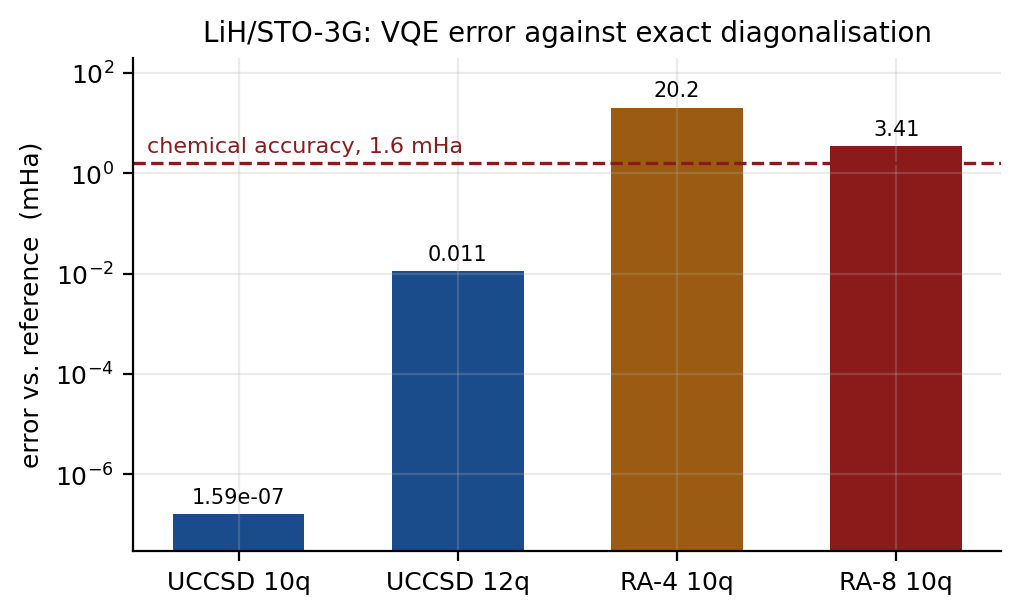
\includegraphics[width=0.74\textwidth]{figures/lih-error.png}
\caption{Error against exact diagonalisation, logarithmic. The two UCCSD runs
clear chemical accuracy by six orders of magnitude and by a factor of $145$
respectively. Read alone, this figure says the eight-layer hardware-efficient
run is the better of the two \code{real\_amplitudes} results;
Figure~\ref{fig:contam} says otherwise.}
\label{fig:error}
\end{figure}

UCCSD at 10 qubits converges in ten L-BFGS-B iterations and twelve objective
evaluations. The residual $1.59\times10^{-7}\mHa$ is not an ansatz limitation:
CASCI(2e,5o) with two electrons is within the reach of singles and doubles
exactly, and what remains is optimiser tolerance. At 12 qubits the residual
rises to $0.011\mHa$, still a factor of $145$ inside the threshold, and the
floor there is finite-difference gradient noise rather than expressivity.

\subsection{The symmetry audit}

\begin{table}[htbp]
\centering
\caption{Symmetry diagnostics at the converged state. \emph{Priced} is the
contamination energy at $1\Ha$ per unit, against the $0.16\mHa$ budget of
\S\ref{sec:criteria}.}
\label{tab:symmetry}
\small
\begin{tabular}{llrrrr}
\toprule
Ansatz & Space & $\Nop - N$ & \Ssq & Priced (mHa) & Verdict \\
\midrule
UCCSD & 10q & $1.0\times10^{-13}$ & $2.60\times10^{-9}$ & $0.0000026$ & inside \\
UCCSD & 12q & $8.4\times10^{-13}$ & $1.37\times10^{-7}$ & $0.000137$  & inside \\
RA-4  & 10q & $3.2\times10^{-8}$  & $3.46\times10^{-10}$ & $0.000064$ & inside \\
RA-8  & 10q & $7.1\times10^{-5}$  & $2.05\times10^{-3}$ & $\mathbf{2.191}$ & \textbf{outside} \\
\bottomrule
\end{tabular}
\end{table}

\begin{figure}[htbp]
\centering
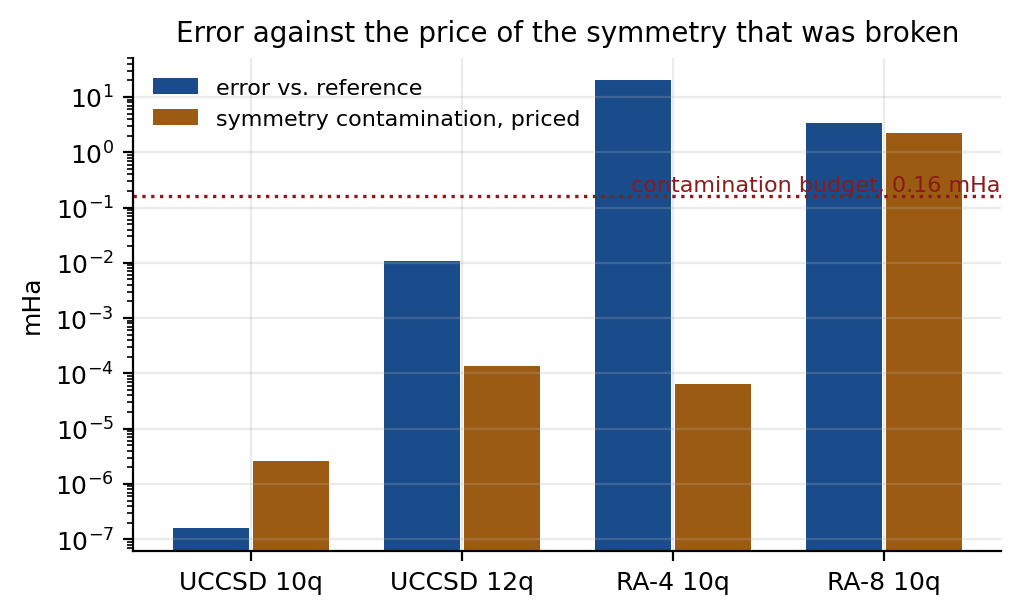
\includegraphics[width=0.74\textwidth]{figures/lih-contamination.png}
\caption{Error beside the price of the symmetry that was broken to obtain it.
For the first three runs the contamination is orders of magnitude below the
error, and the error is therefore a statement about the ansatz. For RA-8 the
contamination exceeds the error.}
\label{fig:contam}
\end{figure}

This is the central observation of the report. Doubling the depth of the
hardware-efficient circuit from four layers to eight moves the energy from
$20.15\mHa$ to $3.41\mHa$ above the reference. Presented as Table~\ref{tab:runs}
alone, that is a sixfold improvement and reads as progress toward chemical
accuracy: another doubling would appear to be all that is required.

Table~\ref{tab:symmetry} shows what actually happened. The eight-layer circuit
bought its energy by leaving the two-electron singlet sector. Its
particle-number deviation is three orders of magnitude larger than the
four-layer run's, its $\Ssq$ is seven orders larger, and together these price at
$2.191\mHa$ --- $13.7$ times the budget, and $0.79\mHa$ \emph{more} than the
error it claims to have left. There is no residual against which to compare a
further improvement, because the quantity being reported is not an energy of
LiH in the target sector.

The four-layer run, which by the energy alone looks like the failure, is the
scientifically usable measurement of the two: its contamination is
$6.4\times10^{-5}\mHa$, so its $20.15\mHa$ error is an honest statement that a
four-layer linear-entanglement \code{real\_amplitudes} circuit recovers
essentially none of the correlation energy of this system. The audit inverts the
ordering of the two runs.

\begin{unsupported}[What Table~\ref{tab:runs} would say without Table~\ref{tab:symmetry}]
``Increasing \code{real\_amplitudes} depth from four to eight layers reduces the
error against CASCI by a factor of $5.9$, to $3.41\mHa$, suggesting that
chemical accuracy is reachable with a hardware-efficient ansatz at modest
additional depth.'' Every number in that sentence is correct. The conclusion
does not follow.
\end{unsupported}

\subsection{Cost}

\begin{figure}[htbp]
\centering
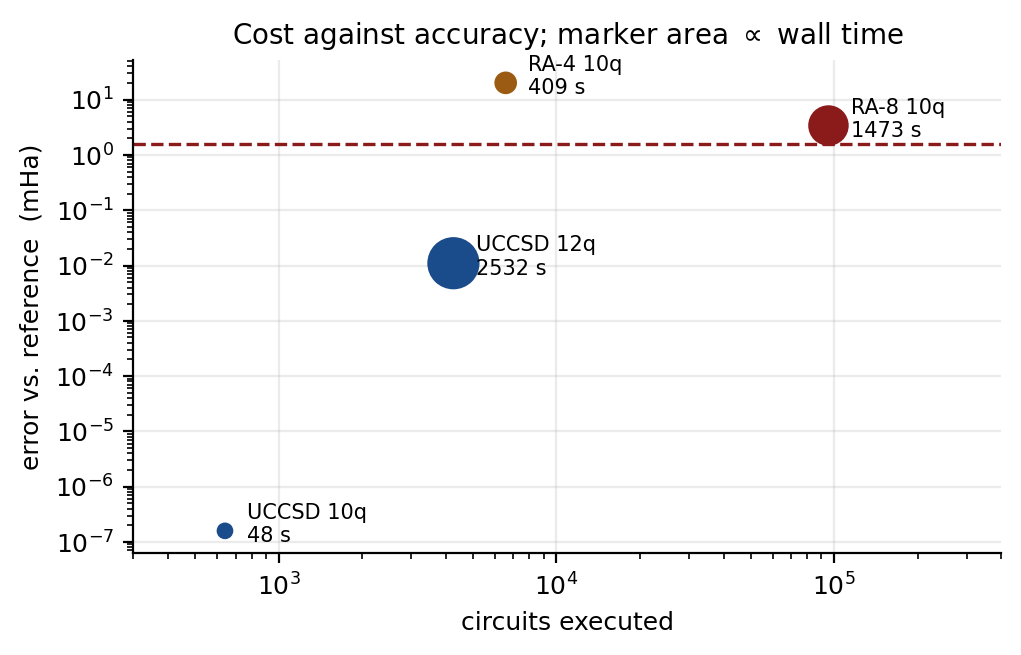
\includegraphics[width=0.74\textwidth]{figures/lih-cost.png}
\caption{Circuit executions against error; marker area proportional to wall
time. The two families are separated by roughly two orders of magnitude in cost
at every accuracy.}
\label{fig:cost}
\end{figure}

The cost asymmetry is as large as the accuracy asymmetry and has the same
cause. UCCSD converges in $10$ and $18$ optimiser iterations respectively
because its doubles amplitudes have a finite gradient at the Hartree--Fock
reference --- the same quantity that makes MP2 non-zero. The hardware-efficient
circuit does not: at $\theta = 0$ it \emph{is} the Hartree--Fock determinant,
and because the Hamiltonian conserves particle number, a lone $R_y$ excitation
out of that determinant has exactly zero gradient. Measured live-parameter
counts at $\theta = 0$ are $0/50$ in the frozen-core space and $0/60$ in the
full space; L-BFGS-B started there returns after zero iterations reporting clean
convergence at $E_{\mathrm{HF}}$.

The workaround is a Gaussian kick, and its magnitude is not a free parameter.
Measured on the self-test's synthetic two-electron 10-qubit system with four
layers:

\begin{table}[htbp]
\centering
\caption{Initialisation study, \code{real\_amplitudes}, four layers, L-BFGS-B to
convergence.}
\label{tab:start}
\small
\begin{tabular}{ll}
\toprule
Start & Result \\
\midrule
$\theta = 0$ exactly        & $0$ iterations, stuck at $E_{\mathrm{HF}}$ \\
$\theta = 0 + N(0, 0.05)$   & converges, $0.0\%$ of correlation recovered \\
$\theta = 0 + N(0, 0.2)$    & converges, $0.0\%$ recovered \\
$\theta = 0 + N(0, 0.5)$    & converges $2.20\Ha$ \emph{above} $E_{\mathrm{HF}}$ \\
uniform $[-\pi, \pi]$       & fails to converge, $1.29\Ha$ above $E_{\mathrm{HF}}$ \\
\bottomrule
\end{tabular}
\end{table}

Near $\theta = 0$ the landscape is flat; further out it is populated with high
local minima. A larger kick is not a better one. On real LiH the default
$\sigma = 0.05$ does let the optimiser move, and it still recovers essentially
none of the correlation --- so the limitation is the ansatz, not the start, and
that conclusion required distinguishing the two.

\subsection{Simulator method}

\code{matrix\_product\_state} is the package default because it is the method
that scales to the larger active spaces this workflow is a warm-up for, and
because \code{vqe} re-evaluates its converged energy with \code{statevector} and
refuses to claim accuracy if the two disagree. At \emph{this} size it is not the
fast choice. Measured on this machine at 10 qubits with an ${\sim}880$-term
objective, one L-BFGS-B iteration of $101$ circuits over $50$ parameters:

\begin{center}
\small
\begin{tabular}{lr}
\toprule
Method & Per iteration \\
\midrule
\code{matrix\_product\_state} & ${\sim}13$ s \\
\code{statevector}            & ${\sim}2.4$ s \\
\bottomrule
\end{tabular}
\end{center}

MPS pays a per-Pauli-term contraction cost that a 10-qubit statevector does not
have, and UCCSD's much deeper circuits widen the gap. Every run in
Table~\ref{tab:runs} therefore used \code{statevector}, and
\code{mps\_vs\_statevector\_hartree} is recorded as exactly $0.0$ in each result
file.

% ============================================================ DISCUSSION ====
\section{Discussion}

\subsection{Why the audit is cheap and the failure is not}

Measuring $\Nop$ and $\Ssq$ at the converged state costs two expectation values
against a run that already executed between $641$ and $95{,}391$ circuits. In
the worst case here the instrumentation is a $2\times10^{-5}$ fraction of the
computation it validates. The failure it catches, by contrast, is silent: the
optimiser converged cleanly, the energy moved in the right direction, and the
number produced lies in a plausible range. Nothing in the optimisation reports a
problem, because from the optimiser's point of view there is none --- it
minimised the objective it was given, over the whole Hilbert space, and the
objective's lower bound over that space is below the sector ground state.

\subsection{Why UCCSD does not need the apparatus}

UCCSD is built from fermionic excitation operators with balanced creation and
annihilation indices, so it commutes with $\hat N$ and $\hat S_z$ exactly. The
number penalty contributes identically zero, and the measured leak at the
optimum is $-1.3\times10^{-15}$ in the frozen-core space. The penalty machinery
is still applied and still audited; it simply has nothing to correct.

This is worth stating precisely, because the guarantee is narrower than it is
often taken to be. UCCSD conserves $N$ and $S_z$ but \emph{not} $S^2$ at
arbitrary amplitudes, since its $\alpha \to \alpha$ and $\beta \to \beta$
amplitudes are independent. It becomes a spin eigenstate at the variational
minimum, which is where $\Ssq$ is measured --- and Table~\ref{tab:symmetry}
records $2.6\times10^{-9}$ and $1.4\times10^{-7}$, consistent with that
expectation but not guaranteed by construction.

\subsection{What the self-test does and does not establish}

\code{run.py selftest} proves the stack: operator conversion checked both
spectrally and determinant by determinant (the latter is what pins down qubit
ordering, since a bit permutation is a similarity transform and leaves the
spectrum unchanged), the Hartree--Fock frame rotation, MPS against exact
statevector, parameter shift against finite differences, and the requirement
that the VQE respect the variational bound, terminate cleanly and never return a
point worse than its own start.

It does \emph{not} assert that the VQE reaches the exact answer or beats
Hartree--Fock. Its Hamiltonian is random, and per Table~\ref{tab:start} the
hardware-efficient ansatz genuinely cannot solve it at this filling. A self-test
demanding otherwise would be asserting expressivity it cannot promise.
Correlation recovery is printed there as a diagnostic and is not scored. For the
claim that the chemistry is right, the evidence is
\code{tests/test\_integrals.py} and \code{run.py validate}.

% ========================================================== UNSUPPORTED =====
\section{Claims not supported by these data}
\label{sec:unsupported}

\begin{enumerate}[leftmargin=1.4em,itemsep=0.3em]

\item \textbf{That \code{real\_amplitudes} cannot reach chemical accuracy on
  LiH at any depth.} Two depths were run. The eight-layer result is
  uninterpretable for the reason given above, so the evidence is a single valid
  point. Deciding this needs a depth scan with the number penalty raised to a
  validated value at each depth, and \Ssq\ recorded throughout.

\item \textbf{That the eight-layer circuit would reach chemical accuracy if the
  penalty were raised.} Plausible and untested. Raising \code{--number-penalty}
  requires re-running \code{validate} at the new value, and the run was not
  repeated.

\item \textbf{That $3.41\mHa$ is an upper bound on what the eight-layer circuit
  can achieve.} The run stopped on \code{TOTAL NO. OF ITERATIONS REACHED LIMIT}
  at $500$ iterations, not on convergence. It was still descending.

\item \textbf{Anything about hardware.} Every number here is a noiseless
  simulation. No shot noise, no readout error, no decoherence, no transpilation
  to a physical coupling map.

\item \textbf{That the STO-3G numbers approximate experiment.} They approximate
  exact diagonalisation in STO-3G, which is roughly $1$ kcal/mol from the
  basis-set limit for LiH.

\end{enumerate}

% ============================================================ LIMITATIONS ===
\section{Limitations}

\begin{enumerate}[leftmargin=1.4em,itemsep=0.2em]
\item One geometry. No potential-energy curve, so no dissociation energy and no
  test of whether the conclusions survive into a multireference regime --- which
  for LiH they would not be expected to at $1.595\Ang$.
\item One basis. The integral engine is STO-3G only by construction.
\item Seed $7$ throughout; no statistics over initialisations for the
  hardware-efficient runs, whose outcome is initialisation-dependent by
  Table~\ref{tab:start}.
\item The $1\Ha$ per unit contamination price is a convention. It is stated so
  that the budget can be recomputed under a different one, not derived.
\item The RA-4 circuit count is recorded as approximate in the source table;
  the exact figure is not in the result file, which stores
  \code{aer\_batches: 66} and the batch composition rather than a total.
\end{enumerate}

% ============================================================ CONCLUSIONS ===
\section{Conclusions}

\begin{enumerate}[leftmargin=1.4em,itemsep=0.25em]

\item UCCSD solves LiH/STO-3G to $1.6\times10^{-7}\mHa$ at 10 qubits and
  $0.011\mHa$ at 12 qubits against exact diagonalisation of the identical
  Hamiltonian, with structurally conserved particle number.

\item The molecular integrals were produced without an external quantum
  chemistry package, by an engine pinned against published RHF and FCI energies
  and against the requirement that the second-quantised Hamiltonian reproduce
  the SCF energy on the reference determinant to ten decimals.

\item A hardware-efficient circuit at eight layers reaches $3.41\mHa$ and the
  number is not usable. Its symmetry contamination prices at $2.19\mHa$ against
  a $0.16\mHa$ budget --- more than the error it has left. The four-layer run,
  worse by a factor of six, is the valid measurement of the two.

\item The instrumentation that decides this is two expectation values on the
  converged state. Against a run of $95{,}391$ circuits, that is not a cost.
  Without it, Table~\ref{tab:runs} supports a conclusion that
  Table~\ref{tab:symmetry} refutes.

\end{enumerate}

% ============================================================== APPENDIX ====
\appendix

\section{Provenance digests}

Every result file records the SHA-256 of the cache it read, the molecular
specification, and the workflow source that produced it. A mismatch is a hard
error, not a warning.

\begin{center}
\small
\begin{tabular}{ll}
\toprule
Quantity & Digest (first 16 hex) \\
\midrule
Frozen-core specification  & \code{2c2041c7740e08d7} \\
Frozen-core cache          & \code{6423e19956432afc} \\
Full-space specification   & \code{e48966a0f0827801} \\
Full-space cache           & \code{b6e5122d87dd5be9} \\
Chemistry workflow         & \code{b5eed0d532b10fcb} \\
Validation workflow        & \code{04b2e651dd029c5b} \\
Runtime workflow (RA-8, UCCSD-12q) & \code{da1c3cda75f59681} \\
\bottomrule
\end{tabular}
\end{center}

\section{Complete settings}

\begin{center}
\small
\begin{tabular}{ll}
\toprule
Setting & Value \\
\midrule
Optimiser                    & L-BFGS-B \\
Tolerance                    & $10^{-10}$ \\
Maximum iterations           & $500$ \\
Seed                         & $7$ \\
Simulator method             & \code{statevector} \\
MPS truncation threshold     & $10^{-16}$ (unused) \\
Hamiltonian cutoff           & $10^{-6}\Ha$ \\
Number penalty               & $1.0\Ha$ \\
Spin penalty                 & $0.0\Ha$ \\
Contamination price          & $1.0\Ha$ per unit \\
Contamination budget         & $1.6\times10^{-4}\Ha$ \\
UCCSD gradient               & central finite difference \\
\code{real\_amplitudes} gradient & parameter shift \\
\code{real\_amplitudes} start    & $\theta=0 + N(0,0.05)$ \\
UCCSD start                  & $\theta = 0$ exactly \\
\bottomrule
\end{tabular}
\end{center}

\section{Software environment}

Python 3.12.13 on Windows 11. qiskit 2.5.2, qiskit-aer 0.17.2, qiskit-nature
0.8.0, OpenFermion 1.8.1, NumPy 2.5.2, SciPy 1.18.0. PySCF absent; integrals
from the native engine.

\section{Reproduction}

\begin{verbatim}
uv venv --python 3.12 .venv && .venv\Scripts\activate
uv pip install -r requirements.txt

python run.py selftest
python run.py prepare
python run.py validate
python run.py vqe --ansatz uccsd --method statevector --start-noise 0

python run.py prepare  --space full
python run.py validate --space full
python run.py vqe --space full --ansatz uccsd \
                  --method statevector --start-noise 0

python run.py vqe --ansatz real-amplitudes --layers 4 --method statevector
python run.py vqe --ansatz real-amplitudes --layers 8 --method statevector

python -m unittest discover -s tests
\end{verbatim}

\section{Data inventory}

\begin{center}
\small
\begin{tabular}{ll}
\toprule
File & Contents \\
\midrule
\code{lih\_frozen\_core\_hamiltonian.json}       & CASCI(2e,5o) cache, 276 Pauli terms \\
\code{lih\_frozen\_core\_hamiltonian.json.validated.json} & its receipt \\
\code{lih\_full\_hamiltonian.json}               & FCI(4e,6o) cache, 631 Pauli terms \\
\code{lih\_full\_hamiltonian.json.validated.json} & its receipt \\
\code{lih\_frozen\_core\_vqe\_result.json}       & UCCSD, 10 qubits \\
\code{lih\_full\_vqe\_uccsd.json}                & UCCSD, 12 qubits \\
\code{lih\_frozen\_core\_vqe\_hea4.json}         & \code{real\_amplitudes}, 4 layers \\
\code{lih\_frozen\_core\_vqe\_hea8.json}         & \code{real\_amplitudes}, 8 layers \\
\bottomrule
\end{tabular}
\end{center}

All eight files live beside \code{run.py} and are committed, so every number in
this report is recomputable from the repository without re-running anything.

\section*{References}
\small
\begin{enumerate}[leftmargin=1.4em,itemsep=0.1em]
\item K.\ P.\ Huber and G.\ Herzberg, \emph{Molecular Spectra and Molecular
  Structure IV: Constants of Diatomic Molecules}, via NIST CCCBDB.
\item A.\ Szabo and N.\ S.\ Ostlund, \emph{Modern Quantum Chemistry}, Dover,
  1996 --- H$_2$/STO-3G reference energies.
\item L.\ E.\ McMurchie and E.\ R.\ Davidson, \emph{J.\ Comput.\ Phys.}
  \textbf{26}, 218 (1978) --- the integral recursion used by
  \code{integrals.py}.
\end{enumerate}

\end{document}
